\documentclass[sigconf,anonymous,review]{acmart}

\usepackage{amsmath,amssymb}
\usepackage{booktabs}
\usepackage{graphicx}
\usepackage{subcaption}
\usepackage{xspace}

\newcommand{\system}{\textsc{MatchShard}\xspace}
\newcommand{\ctx}{\textsf{CTX}\xspace}
\newcommand{\sid}{\mathsf{sid}}

\title{Match, Aggregate, Settle: Compressing Cross-Shard Execution for Web3 Transactions}

\author{Anonymous Authors}

\begin{document}

\begin{abstract}
Cross-shard transactions are indispensable to Web3 applications, yet current sharded blockchains still carry their destination-side effects one transaction at a time. This transaction-granular path duplicates relay messages, block entries, verification, and state-access work when many finalized source-side transfers update the same destination shard or account. We present \system, a cross-shard execution protocol that separates source-side finality from destination-side materialization. Source shards validate and debit payers, then send compact, authenticated summaries to a coordination chain. A new pre-matching stage cheaply screens and indexes eligible summaries before an exact matcher selects the largest feasible set. The coordinator aggregates selected receiver-side deltas---including many source shards paying the same account---and emits one or a few verifiable settlement transactions; unselected summaries retain the ordinary relay path. We state the protocol invariants for authorization, conservation, exactly-once application, and fallback liveness, and implement the design in BlockEmulator-X. Across 4--24 shards and five repeated runs, \system improves throughput by 22.8--110.6\% and reduces mean confirmation latency by 22.1--83.9\% relative to relay, broker, and workload-partitioning baselines. At eight shards, its 95th-percentile confirmation latency is 14.6\,s, versus 50.5--52.0\,s for the baselines, while coordination accounts for 2.50\,s of the 8.69\,s mean. These results show that receiver-side aggregation is a practical complement to faster consensus and better account placement.
\end{abstract}

\maketitle

\section{Introduction}

Sharding lets a blockchain execute independent workloads in parallel, and is therefore a foundation for scalable decentralized-Web infrastructure~\cite{elastico2016,omniledger2018,rapidchain2018,monoxide2019}. Its hardest remaining path is a transaction whose payer and receiver live on different shards. Such cross-shard transactions are common in Web3 exchanges, games, marketplaces, and agent-mediated payments, where users and contracts cannot be kept permanently co-located. Existing protocols make this path safe and increasingly fast~\cite{chainspace2018,rivet2020,logos2026,xrbc2026,lightcross2024,presto2024}, but generally preserve one receiver-side execution item per transfer.

That granularity is expensive. After a source shard has authenticated a payer and finalized a debit, the destination still receives a message, consumes block space, verifies evidence, and updates state for every transfer. Under skewed traffic, the destination queue grows even when many items target the same shard or account. Account migration and workload-aware placement reduce how often the path is taken~\cite{spring2024,finelock2024,statesharding2024,mvss2024,shardscheduler2021,txallo2022}; they do not compress cross-shard effects that remain.

Figure~\ref{fig:motivation} exposes the resulting asymmetry. Source shards already validate and order the outgoing CTXs through their local consensus, yet a transaction-granular protocol materializes all $k+m$ receiver-side effects again at the destinations. The proposed path moves the cross-shard coordination result into compact settlement transactions. A matched group therefore occupies one settlement entry per involved shard, while the residual that cannot enter the group follows the fallback path. This change attacks the repeated destination work directly: it reduces the number of destination entries without bypassing source-side consensus.

\begin{figure}[t]
    \centering
    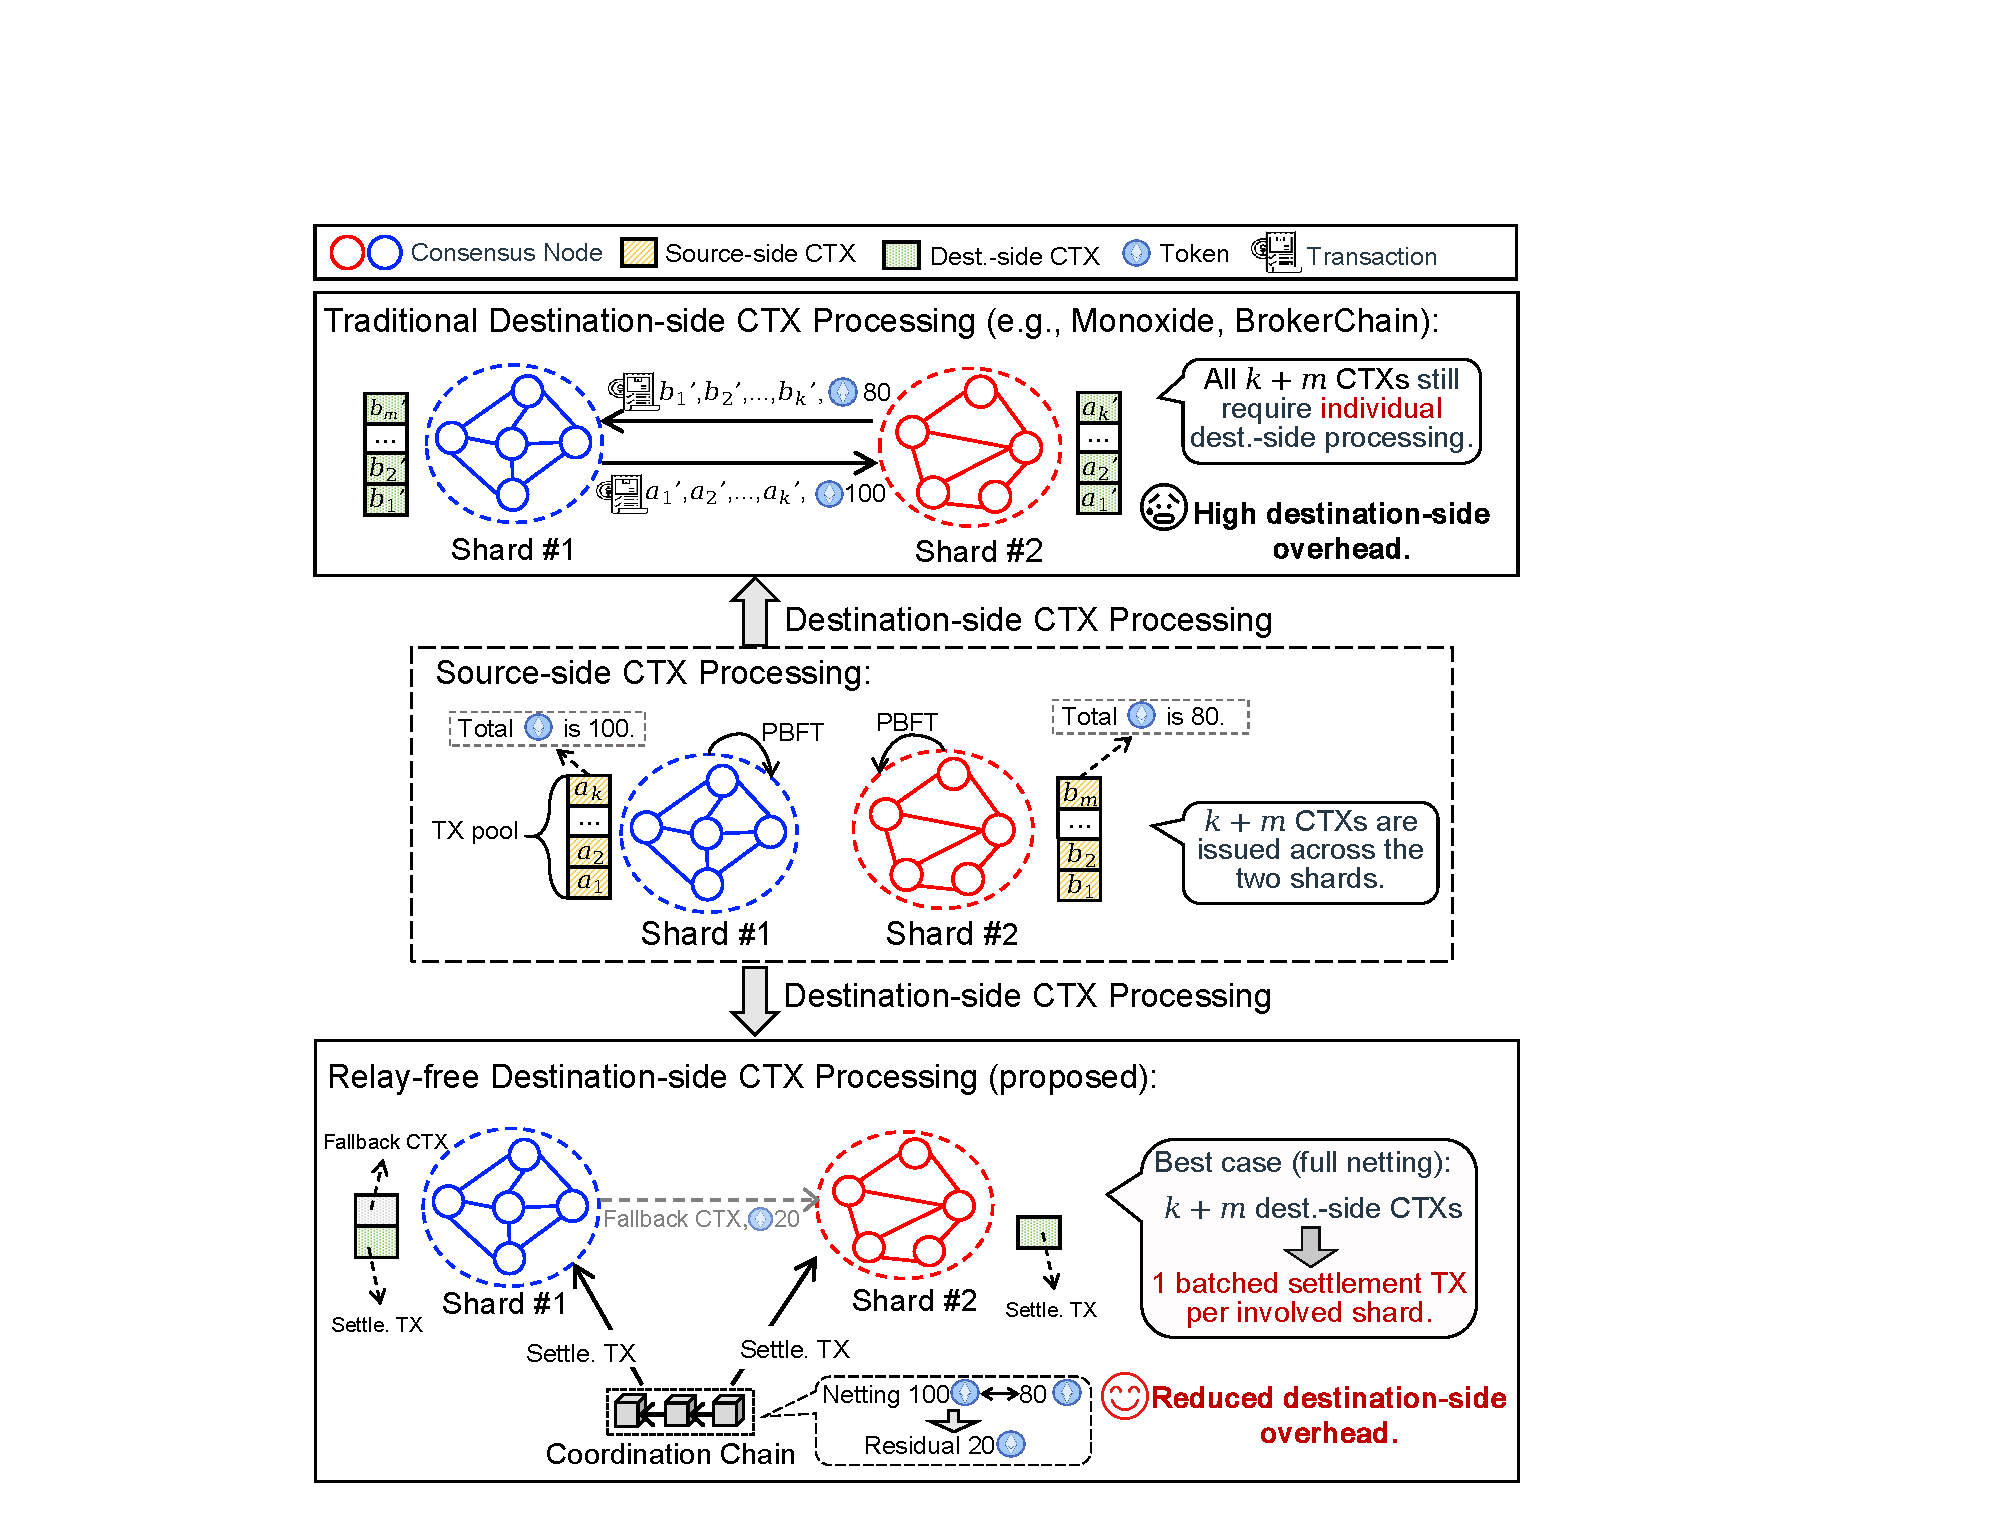
\includegraphics[width=\linewidth]{Fig1.pdf}
    \caption{Why transaction-granular cross-shard execution wastes destination capacity. Traditional relay and broker protocols materialize all $k+m$ CTXs individually after source-side consensus. Matching converts the compatible portion into a compact settlement transaction for each involved shard; the unmatched residual uses a fallback CTX.}
    \label{fig:motivation}
\end{figure}

This paper asks a different question: \emph{after payer-side effects are final, how few destination-side execution items are necessary to preserve the same receiver balances?} For additive transfers, receiver updates commute. A coordinator can match compatible finalized summaries across the two directions of a shard pair, combine the selected credits by destination account, and materialize the result with compact settlement transactions. Matching determines which CTXs share a settlement; aggregation then coalesces their receiver updates, including many-to-one traffic in which several source accounts pay the same destination account. Every selected CTX remains committed by identifier, while the unmatched residual retains its individual fallback path.

The idea creates three nontrivial requirements. First, matching every pending item exactly is wasteful when most candidates are incompatible, so the system needs a cheap stage that reduces the search space without changing ledger state. Second, aggregation must remain auditable: a destination must be able to derive the included transfers and reject omissions, duplication, or altered amounts. Third, optimization cannot endanger progress; anything not selected must complete through an established fallback path.

We address these requirements with \system. Each source shard finalizes the sender-side effect and exports a signed summary to a Beacon Chain. The Beacon Chain performs \emph{pre-matching}: it rejects stale or malformed items, groups candidates by settlement compatibility, maintains lightweight account and shard indexes, and estimates whether a group merits exact optimization. The exact matcher then selects a feasible set that maximizes the number of aggregated summaries subject to capacity and deadline constraints. Aggregation folds the chosen credits by receiver, after which settlement transactions commit the resulting updates and an inclusion digest. Residual summaries fall back to relay without re-executing the debit. Figure~\ref{fig:system-overview} shows the complete execution path: source shards reserve and finalize CTXs, the matching coordinator constructs the selected set and its commitment, the Beacon Chain finalizes the commitment, and settlement contracts apply the receiver updates at both shards.

\begin{figure*}[t]
    \centering
    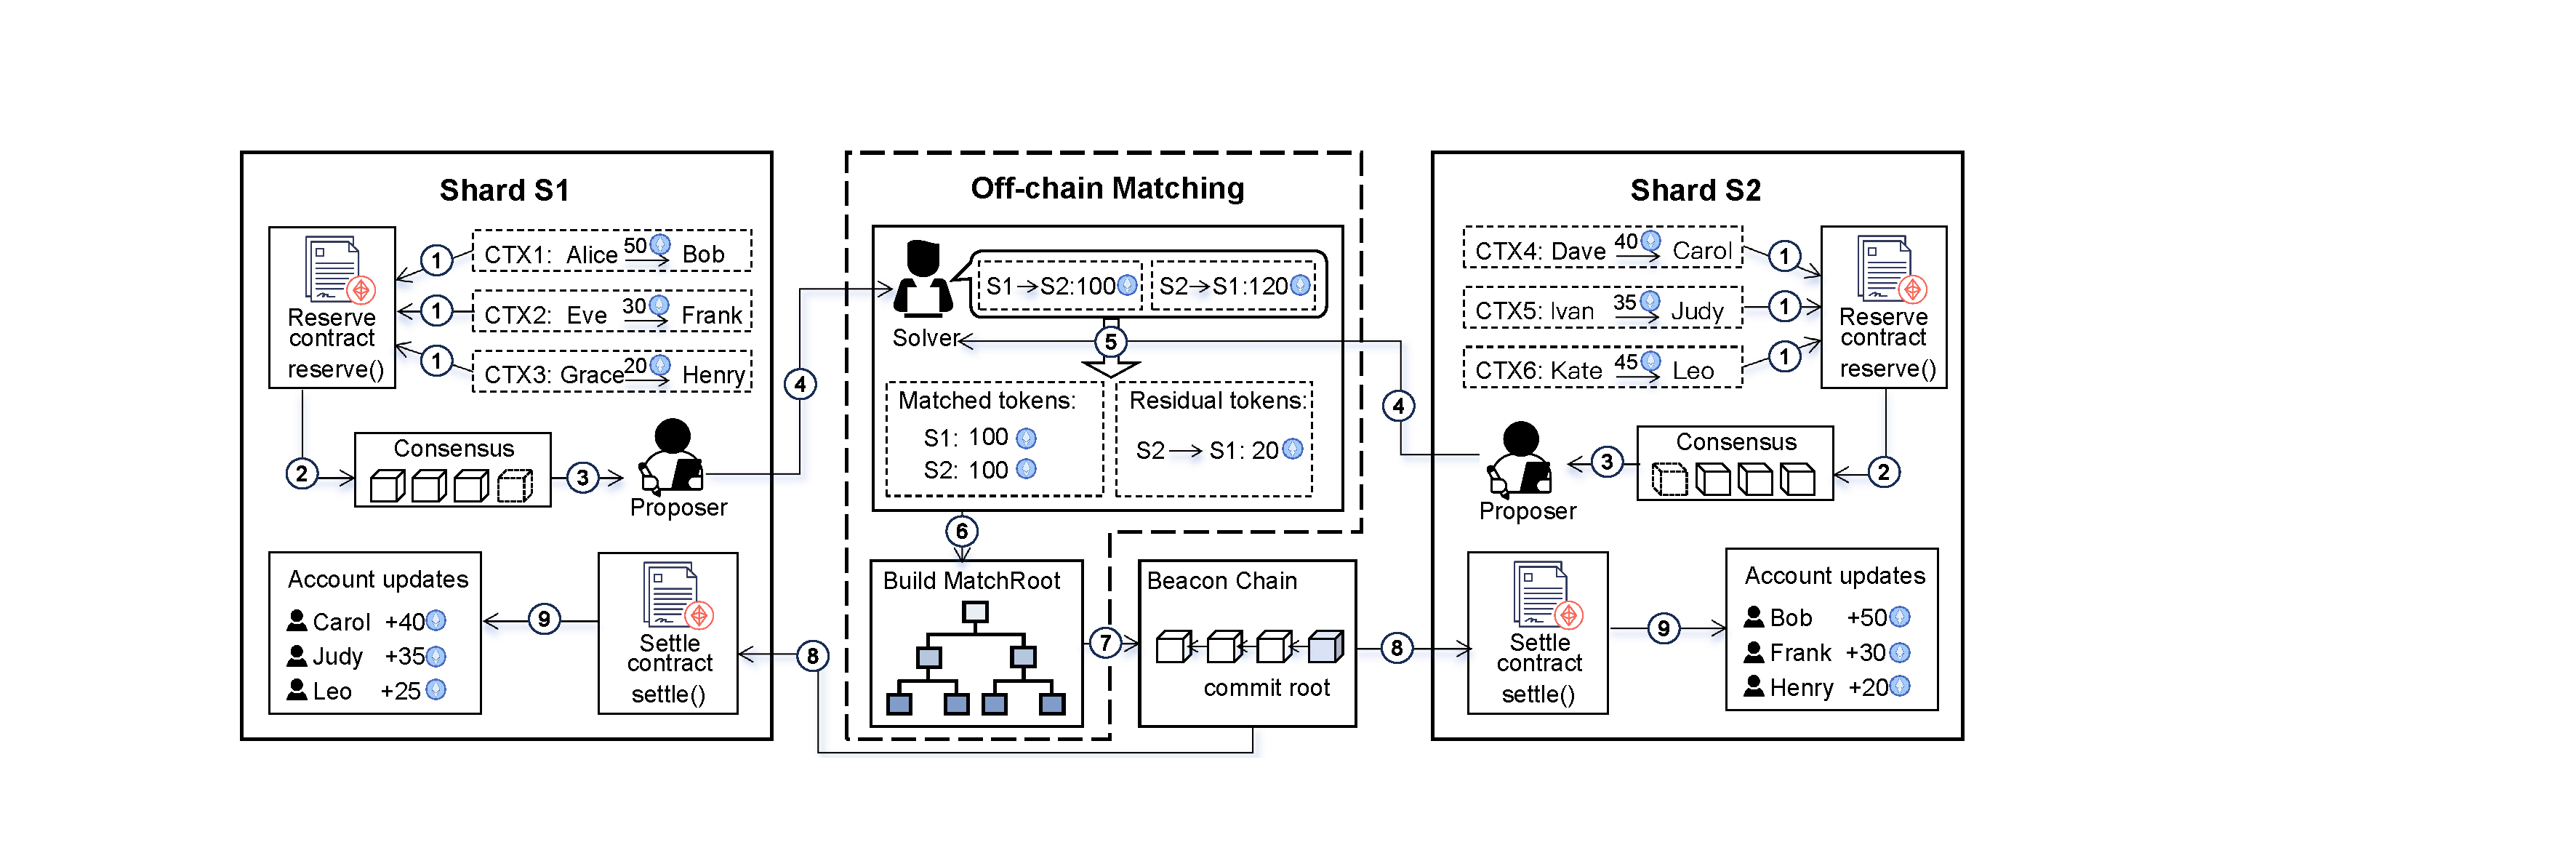
\includegraphics[width=.98\textwidth]{Fig2.pdf}
    \caption{System workflow of \system. Source shards reserve outgoing CTXs and finalize them through local consensus (Steps 1--4). The coordinator performs pre-matching and exact matching, separates selected and residual CTXs, and constructs a \emph{MatchRoot} (Steps 5--6). The Beacon Chain commits the root (Step 7), after which settlement contracts verify the commitment and apply the receiver-side account updates (Steps 8--9). Residual CTXs retain the fallback path.}
    \label{fig:system-overview}
\end{figure*}

\paragraph{Preliminary evidence.}
The design is driven by two measured properties of the workload. First, matching opportunities are abundant and remain available as the system scales. Figure~\ref{fig:pre-matchability}a shows global matching rates of 74.3\%, 71.8\%, 70.8\%, and 67.4\% as the system grows from 4 to 32 shards; the opportunity remains above 65\% even though additional shards disperse traffic across more pairs. The shard-pair heat map in Figure~\ref{fig:pre-matchability}b further shows strong opportunities across the active matrix instead of a single favorable pair. Together, the two views establish that matching is supported both globally and across individual shard routes.

\begin{figure*}[t]
    \centering
    \begin{subfigure}[t]{.46\textwidth}
        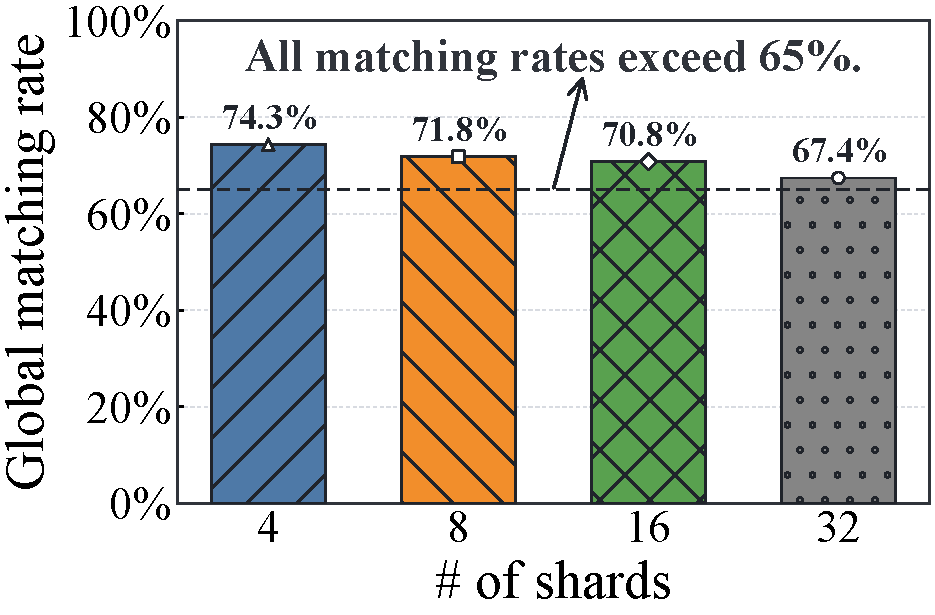
\includegraphics[width=\linewidth]{pre-exp-figs/shard_count_vs_matching_rate.pdf}
        \caption{Scaling the shard count.}
    \end{subfigure}\hfill
    \begin{subfigure}[t]{.46\textwidth}
        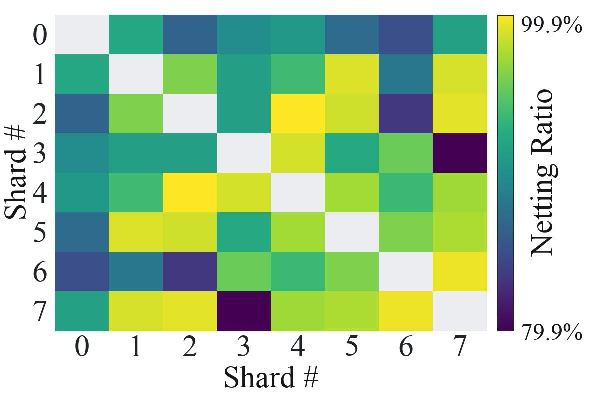
\includegraphics[width=\linewidth]{pre-exp-figs/bidirectional_netting_potential_heatmap.pdf}
        \caption{Opportunities by shard pair.}
    \end{subfigure}
    \caption{Preliminary workload analysis. Matching remains prevalent across shard counts and source--destination pairs.}
    \label{fig:pre-matchability}
\end{figure*}

Second, destination materialization determines system capacity. We run a diagnostic \emph{source-only} configuration that preserves source processing but removes destination-side CTX execution. In Figure~\ref{fig:pre-bottleneck}a, ordinary execution accumulates tens of thousands of queued items at 4K--6K tx/s, whereas source-only processing keeps the queue near the baseline and drains it earlier. Figure~\ref{fig:pre-bottleneck}b shows the consequence: ordinary throughput saturates near 2.8K tx/s and its latency rises sharply with arrival rate, while the source-only diagnostic scales to roughly 4.5K tx/s and maintains low latency. These results identify destination-side repetition as the capacity-limiting work and establish the exact optimization target of \system.

\begin{figure*}[t]
    \centering
    \begin{subfigure}[t]{.48\textwidth}
        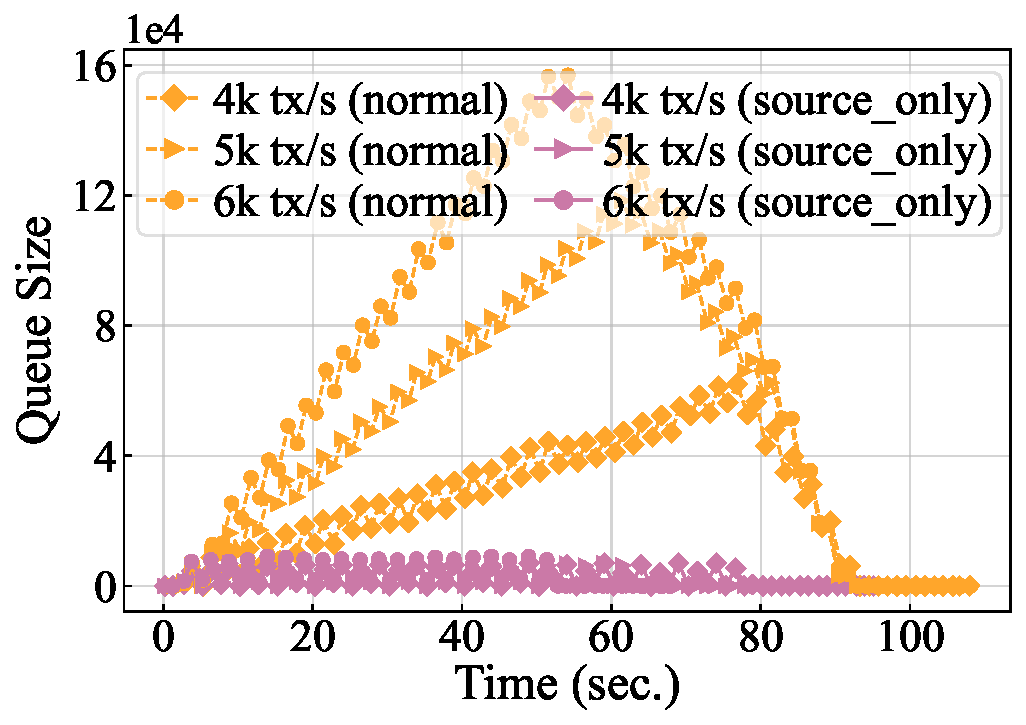
\includegraphics[width=\linewidth]{pre-exp-figs/txpool_total_shards08_six_runs.pdf}
        \caption{Total queue size under increasing load.}
    \end{subfigure}\hfill
    \begin{subfigure}[t]{.48\textwidth}
        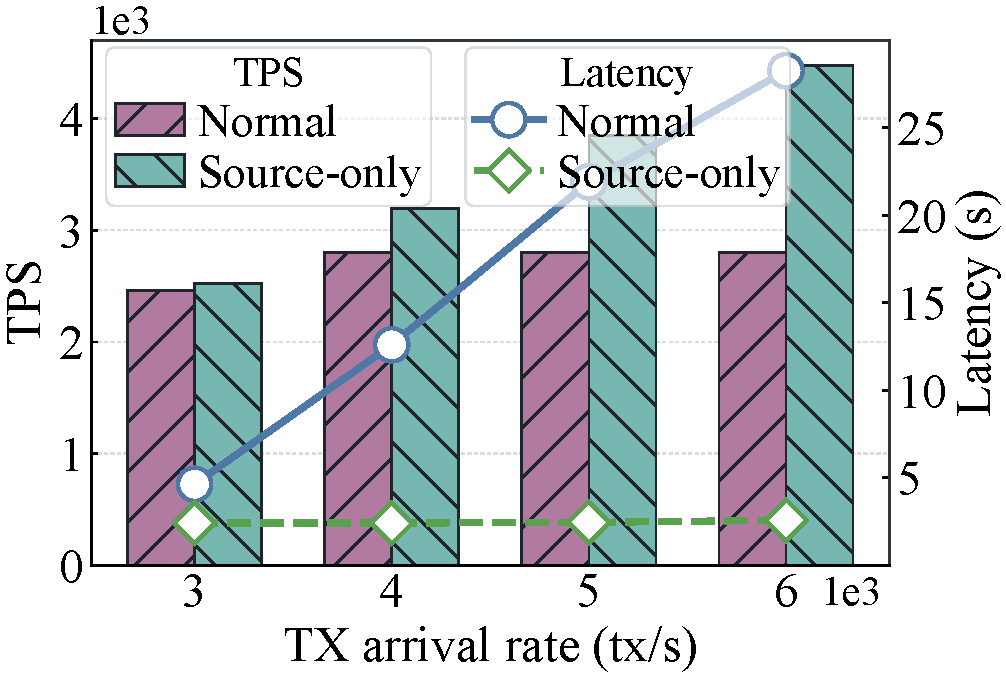
\includegraphics[width=\linewidth]{pre-exp-figs/tps_latency_combo.pdf}
        \caption{Throughput and confirmation latency.}
    \end{subfigure}
    \caption{Preliminary bottleneck diagnosis on eight shards. Removing destination-side materialization eliminates queue growth and exposes the capacity available to a compressed settlement path.}
    \label{fig:pre-bottleneck}
\end{figure*}

This work directly targets the Web's decentralized transaction infrastructure. Its intended track is systems and Web infrastructure: it improves the execution substrate on which Web3 services expose payments and stateful interactions, rather than proposing a cryptocurrency-specific financial primitive. We make four contributions:

\begin{itemize}
  \item We identify destination materialization, rather than only cross-shard consensus, as a compressible bottleneck and formulate selection as maximizing the number of summaries covered by settlement.
  \item We design a pre-matching--matching--aggregation--settlement pipeline that supports many-source-to-one-receiver updates and preserves an ordinary relay fallback.
  \item We provide safety arguments for source authorization, value conservation, deterministic aggregation, and exactly-once destination application.
  \item We implement \system in BlockEmulator-X and evaluate scale, queue pressure, coordination cost, matching coverage, and sensitivity over repeated experiments.
\end{itemize}

\section{Background and Motivation}

\subsection{Transaction-granular cross-shard execution}

Let an account belong to exactly one of shards $\mathcal{S}=\{S_1,\ldots,S_n\}$. For a transfer $t=(a_s,a_d,v,\nu)$, the source shard $src(t)$ verifies the payer, nonce $\nu$, and balance, while $dst(t)$ credits the receiver. Relay protocols carry evidence from source to destination; broker protocols split the path through intermediary accounts~\cite{brokerchain2022,broker2earn2024}; and atomic protocols coordinate the involved partitions~\cite{sharper2021,byshard2021,cerberus2023}. Despite different trust and message structures, these approaches commonly retain $|T_j|$ destination execution items for the set $T_j$ of incoming transfers to $S_j$.

This cost is distinct from bytes on the wire. Every item competes for block capacity, incurs dispatch and verification, touches state, and remains in a queue until proposed. Newer consensus, pipelining, and reliable-broadcast designs lower coordination overhead~\cite{kronos2025,reticulum2024,xrbc2026,cherubim2024,hiba2025,hicocs2025}, but do not remove repeated receiver-side work.

\subsection{Aggregation opportunity}

Once the source-side debit is final, a plain value transfer contributes an additive delta $+v$ to one receiver. For any compatible set $M$, the destination state transition can be written
\begin{equation}
  \Delta_M(a)=\sum_{t\in M:\,a_d(t)=a} v(t).
  \label{eq:aggregate}
\end{equation}
Applying the map $\Delta_M$ once yields the same receiver balances as applying its members individually, provided that every member is authorized and applied exactly once. The number of receiver updates becomes the number of distinct destinations, and the number of block entries becomes the number of bounded-size settlement chunks, rather than $|M|$.

The optimization target is consequently \emph{coverage}, not value cancellation. If $P$ is the pending set and $x_t\in\{0,1\}$ indicates selection, the primary objective is
\begin{equation}
  \max \sum_{t\in P}x_t,
  \label{eq:coverage}
\end{equation}
subject to compatibility, settlement-size, per-shard capacity, and deadline constraints. Maximizing selected summaries equivalently minimizes fallback count. A secondary objective can minimize the number of settlement chunks or balance destination load.

\section{Model and Goals}

\paragraph{Finality and adversary.}
Each shard runs Byzantine fault tolerant consensus and exports a summary only after its source block is final. The Beacon Chain also provides finality. The adversary may delay messages and submit malformed or duplicate summaries, but cannot forge a quorum certificate or revert finalized blocks. Network delivery is eventually synchronous. The consensus assumptions follow practical and responsive BFT protocols~\cite{pbft1999,byzcoin2016,hotstuff2019} and their use in established sharding systems~\cite{omniledger2018,rapidchain2018,chainspace2018}.

\paragraph{Summary.}
A source-finalized summary is
\[
 c_t=\langle \sid_t,src,dst,a_d,v,e,\tau,h_t,QC_{src}\rangle,
\]
where $\sid_t$ is globally unique, $e$ is the execution epoch, $\tau$ is a fallback deadline, $h_t$ commits to the original transaction, and $QC_{src}$ proves the finalized debit. The Beacon Chain stores status $\mathsf{pending}$, $\mathsf{selected}$, $\mathsf{settled}$, or $\mathsf{fallback}$ for each identifier.

\paragraph{Compatibility.}
Two summaries may share a settlement only if they use the same asset and state-transition semantics, have final source proofs, are not expired or previously consumed, and target a destination supported by the settlement chunk. Contract calls with order-dependent side effects remain on the fallback path. This paper focuses on additive account transfers.

\paragraph{Goals.}
The protocol must provide (G1) authorization: no credit without a final source debit; (G2) conservation: settlement preserves every selected amount and receiver; (G3) exactly-once application across settlement and fallback; (G4) liveness: nonselected items eventually complete; and (G5) compression: destination entries and state accesses decrease when compatible groups exist.

\section{Design}

\subsection{Pipeline overview}

\system operates in six stages: source finalization, summary admission, pre-matching, exact matching, aggregation, and settlement/fallback. The crucial separation is that selection never changes account state. Only a destination-finalized settlement or fallback transaction credits a receiver. Consequently, a failed matching round can be retried without undoing payer-side state.

\subsection{Source finalization and admission}

The source shard validates the signature, nonce, balance, and local execution rules, debits or irreversibly reserves $v$, and finalizes the result in a block. It emits $c_t$ rather than forwarding the complete transaction to the destination. The Beacon Chain verifies $QC_{src}$, recomputes the committed identifier, checks epoch and deadline, and rejects identifiers already in its consumed set. Admission changes only coordinator metadata.

This ordering prevents a coordinator from creating value: it can schedule only a credit whose debit is already final. It also prevents concurrent spending because the source shard's ordinary nonce and balance rules serialize payer effects before export.

\subsection{Pre-matching}

Running an exact optimizer over the entire pending pool every round increases coordination latency and makes results sensitive to irrelevant traffic. Pre-matching builds a smaller candidate set using four deterministic filters.

First, an \emph{eligibility filter} removes malformed, expired, unsupported, or already consumed summaries. Second, a \emph{compatibility index} groups the remainder by $(e,asset,dst,semantics)$ and, within each group, by receiver. Third, a \emph{readiness score} estimates the attainable compression from group size, number of repeated receivers, age, and the destination's remaining capacity. Finally, a \emph{candidate gate} sends promising groups and any near-deadline summaries to exact matching. Low-scoring items remain pending until the next window; approaching the deadline gives an item priority and then forces fallback.

Pre-matching is intentionally conservative. A false positive costs matcher time, whereas a false negative only defers an item until a later round or fallback. The stage neither marks an item selected nor authorizes a credit, so approximate scoring cannot violate safety. Its indexes are rebuilt from Beacon state after failure.

\subsection{Exact matching}

For each candidate group $G$, the matcher solves Eq.~\eqref{eq:coverage}. Let $C_d$ be the maximum number of summaries destined for shard $d$ in one round, $B$ the maximum encoded settlement size, and $z_{d,k}$ indicate use of settlement chunk $k$. The constraints include
\begin{align}
 &x_t \leq valid(t), &&\forall t\in G,\\
 &\sum_{t:dst(t)=d}x_t \leq C_d, &&\forall d,\\
 &bytes(d,k)\leq Bz_{d,k}, &&\forall d,k.
\end{align}
The implementation uses deterministic ordering by deadline, destination pressure, and identifier, followed by bounded packing. This provides reproducible selections and makes the optimization cost predictable. The selection record contains the ordered identifiers and is finalized by the Beacon Chain before any settlement is issued.

\subsection{Many-to-one aggregation}

For selected set $M_d$ targeting destination shard $d$, the coordinator computes Eq.~\eqref{eq:aggregate}. Transfers from different source shards to the same account are merged into one receiver delta. The settlement payload contains: the round and destination, a sorted vector of $(account,delta)$ pairs, a Merkle root over selected summaries, source-proof commitments, and a Beacon certificate. Payloads larger than $B$ are deterministically split into chunks, each with disjoint identifiers.

The destination recomputes the inclusion root, verifies the Beacon certificate and source commitments, checks that no identifier is in its local consumed set, and applies all deltas atomically with the consumed-set update. Aggregating by receiver reduces repeated trie or database accesses even when encoding limits require several chunks.

\subsection{Settlement and fallback}

After a destination finalizes a settlement, its receipt is returned to the Beacon Chain, which changes the included identifiers from $\mathsf{selected}$ to $\mathsf{settled}$. An item can enter fallback only while $\mathsf{pending}$ and after its deadline or an explicit rejection. The fallback message reuses the same source proof and identifier, so the destination's consumed set covers both paths. If a selected settlement does not complete, the coordinator reissues the same chunk; it does not create a fallback copy until selection is released by a certified timeout transition.

This design preserves the familiar relay path for sparse, incompatible, or urgent traffic. Matching improves the common case without becoming a liveness dependency.

\section{Correctness and Security}

\textbf{Lemma 1 (source authorization).} Every credited identifier corresponds to one finalized source-side debit. A destination accepts only a source commitment covered by a valid source quorum certificate and a Beacon-certified settlement or fallback message. Unforgeability and shard finality therefore imply the claim.

\textbf{Lemma 2 (aggregation equivalence).} For an accepted settlement set $M$, the post-state receiver balance equals transaction-by-transaction execution in any order. By Eq.~\eqref{eq:aggregate}, each receiver obtains exactly the sum of amounts addressed to it. Addition is associative and commutative, and compatibility excludes order-dependent calls.

\textbf{Lemma 3 (exactly once).} No identifier is applied by both settlement and fallback, or twice by retries. The Beacon status machine permits one active path, while the destination atomically records $\sid_t$ with its credit. Any repeated chunk or fallback request intersects the consumed set and is rejected.

\textbf{Theorem 1 (safety).} Under the stated finality and cryptographic assumptions, \system preserves value and receiver balances relative to individual cross-shard execution. Lemma~1 rules out unsupported credits; Lemma~2 preserves selected receiver effects; Lemma~3 rules out duplication. Unselected items use the original relay semantics.

\textbf{Theorem 2 (eventual completion).} Under eventual synchrony and live shard/Beacon consensus, every admitted summary is eventually settled or falls back. Candidate age raises its priority; a finite deadline prevents indefinite waiting; and the fallback protocol is independent of finding a match.

The coordinator can censor selection but cannot redirect value or mint credits. Persistent censorship becomes ordinary relay after the deadline. Availability of proofs and inclusion identifiers is necessary for auditability; a production deployment can use data-availability sampling or shard receipts, which is orthogonal to the selection algorithm.

\section{Implementation}

We implement \system on BlockEmulator-X~\cite{blockemulatorx2025}, an account-based sharding testbed with PBFT consensus. Consensus nodes process protocol messages serially, which makes settlement and consumed-set updates deterministic. Source leaders export finalized summaries; the supervisor emulates the Beacon Chain and runs pre-matching, deterministic matching, aggregation, and receipt tracking. Settlement transactions enter the ordinary destination transaction pool and are finalized by the same block-production path as baseline transactions.

The implementation maintains indexes keyed by destination shard and receiver, plus a hash set of consumed identifiers. It records source, coordination, and destination timestamps for stage-level measurement. Baselines share the same consensus, block interval, workload, and network configuration. Thus the comparison isolates the cross-shard execution path rather than consensus implementation.

\section{Evaluation}

We answer five questions: (Q1) Does aggregation improve scale-out throughput and latency? (Q2) Is matching coverage high and coordination affordable? (Q3) Where does latency change? (Q4) Does the design relieve queue pressure? (Q5) How sensitive is it to load and matching-window size?

\subsection{Setup}

We compare \system with static relay, static broker, and CLPA relay. CLPA periodically repartitions the account-interaction graph; the broker baseline uses intermediary accounts. Scale experiments use 4, 8, 16, and 24 shards and five independent runs per point. Unless a plot states otherwise, each shard has four PBFT nodes and shares the same block and injection configuration. Error bars report run-to-run variation. Confirmation time is measured from injection to destination finality. The eight-shard distribution and stage breakdown use two 300,000-transaction runs. We report end-to-end results rather than microbenchmarks alone.

\subsection{Q1: Scale-out performance}

\begin{figure}[t]
  \centering
  \begin{subfigure}[t]{0.49\columnwidth}
    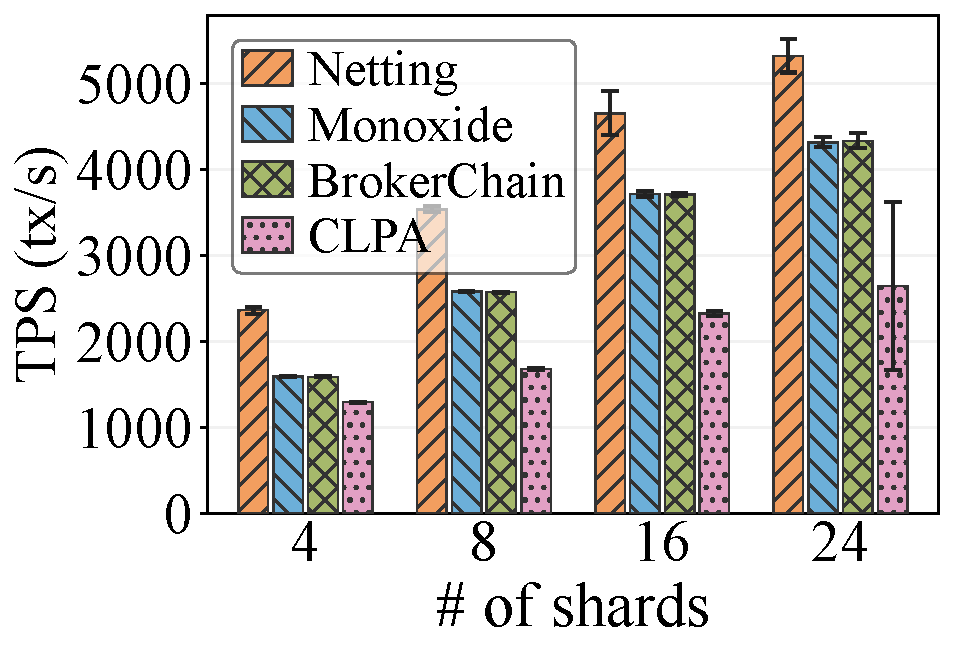
\includegraphics[width=\linewidth]{exp-figs/fig_exp1_scale_tps_bar.pdf}
    \caption{Committed throughput.}
    \label{fig:tps}
  \end{subfigure}\hfill
  \begin{subfigure}[t]{0.49\columnwidth}
    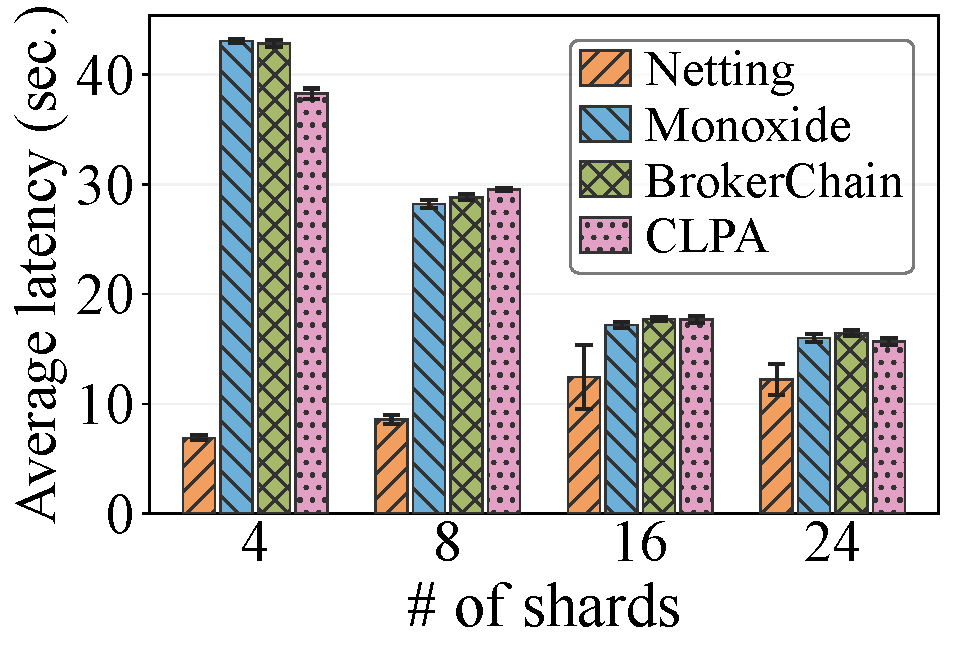
\includegraphics[width=\linewidth]{exp-figs/fig_exp1_scale_latency_bar.pdf}
    \caption{Mean confirmation latency.}
    \label{fig:latency}
  \end{subfigure}
  \caption{Scale-out performance over five runs. \system increases useful throughput while reducing end-to-end latency.}
  \label{fig:scale}
\end{figure}

Figure~\ref{fig:scale} shows that all methods gain throughput with more shards, but transaction-granular destination work limits the baselines. \system commits 2,366, 3,538, 4,656, and 5,325 tx/s at 4, 8, 16, and 24 shards, respectively. Static relay reaches 1,593--4,318 tx/s, static broker 1,592--4,335 tx/s, and CLPA relay 1,296--2,649 tx/s. Depending on scale and baseline, the gain is 22.8--110.6\%. The 24-shard CLPA point has high variance, consistent with repartitioning overhead under the repeated workload.

Latency tells the same story. \system's mean is 6.91, 8.58, 12.44, and 12.23\,s, while the baselines range from 15.70 to 43.04\,s. This is a 22.1--83.9\% reduction. At small scale, removing per-item destination work produces the largest relative benefit; at larger scale, source consensus and injection become a greater fraction of the path.

\subsection{Q2: Coverage and coordination cost}

\begin{figure}[t]
  \centering
  \begin{subfigure}[t]{0.49\columnwidth}
    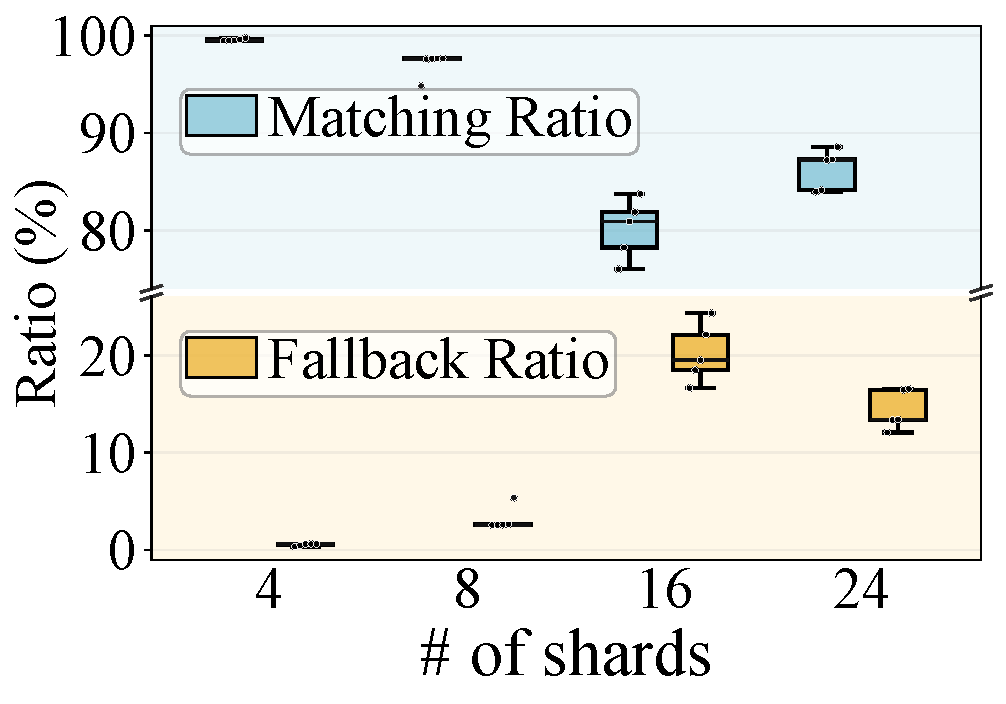
\includegraphics[width=\linewidth]{exp-figs/fig_exp1_scale_matching_fallback_rate_boxplot.pdf}
    \caption{Selected versus fallback share.}
    \label{fig:coverage}
  \end{subfigure}\hfill
  \begin{subfigure}[t]{0.49\columnwidth}
    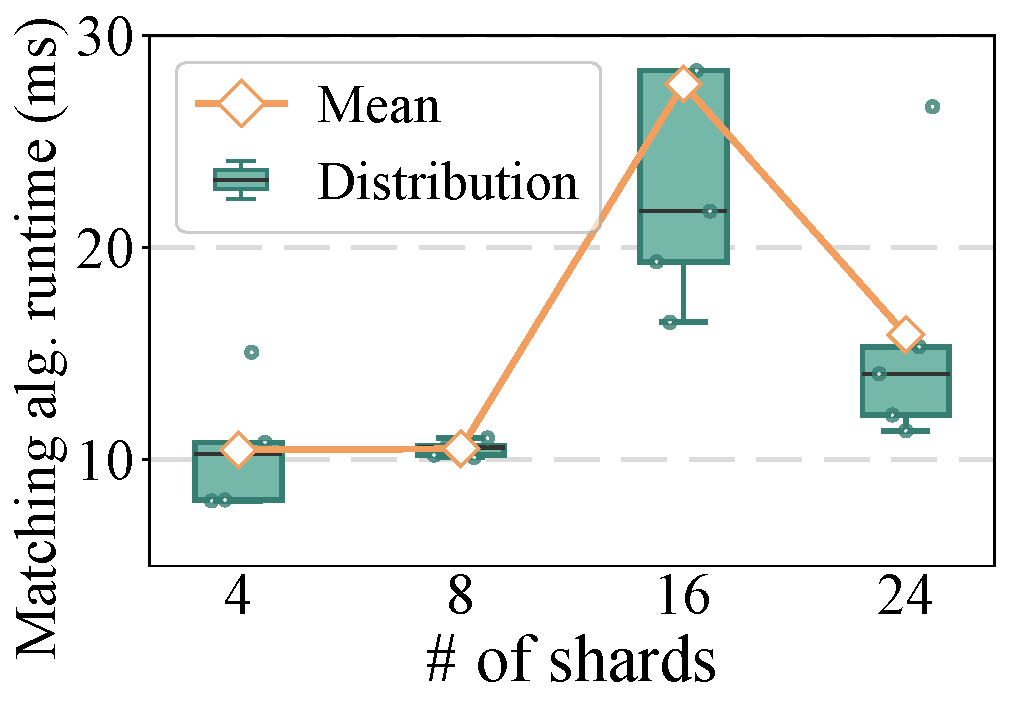
\includegraphics[width=\linewidth]{exp-figs/matching_time.pdf}
    \caption{Coordinator matching time.}
    \label{fig:runtime}
  \end{subfigure}
  \caption{Matching effectiveness and runtime across shard counts. Boxes summarize repeated runs.}
  \label{fig:matchcost}
\end{figure}

Figure~\ref{fig:matchcost} separates algorithmic opportunity from cost. Most eligible summaries are selected, leaving a small fallback fraction across scales. Mean matching runtime is 10.46\,ms at four shards, 10.52\,ms at eight, 27.72\,ms at sixteen, and 15.90\,ms at twenty-four; the largest observed run is 52.70\,ms. The nonmonotonic means reflect candidate composition rather than a direct dependence on shard count: pre-matching groups work by compatibility and destination, so exact optimization sees selected group sizes instead of the entire global pool.

\begin{figure}[t]
  \centering
  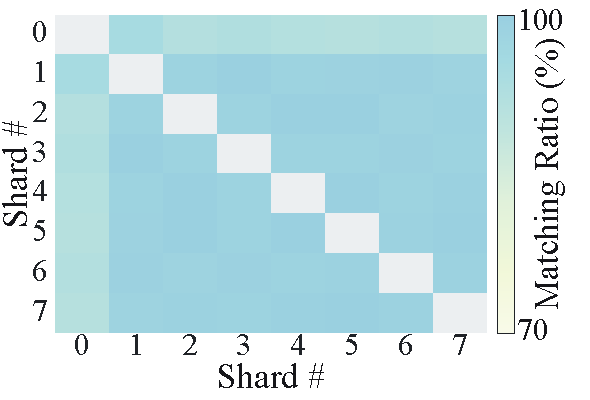
\includegraphics[width=.72\columnwidth]{exp-figs/shard8_matching_rate_heatmap.pdf}
  \caption{Eight-shard source--destination selection rates over five runs. High rates across most shard pairs show that gains do not come from one dominant route.}
  \label{fig:heatmap}
\end{figure}

The pairwise heat map in Figure~\ref{fig:heatmap} provides a stricter view. Across directed shard pairs, rates lie between 91.2\% and 99.4\%. The narrow range indicates that deterministic grouping does not starve lightly represented routes. It also supports the many-source aggregation premise: selection remains high when traffic is divided among multiple source--destination pairs.

\subsection{Q3: End-to-end and stage latency}

\begin{figure}[t]
  \centering
  \begin{subfigure}[t]{0.49\columnwidth}
    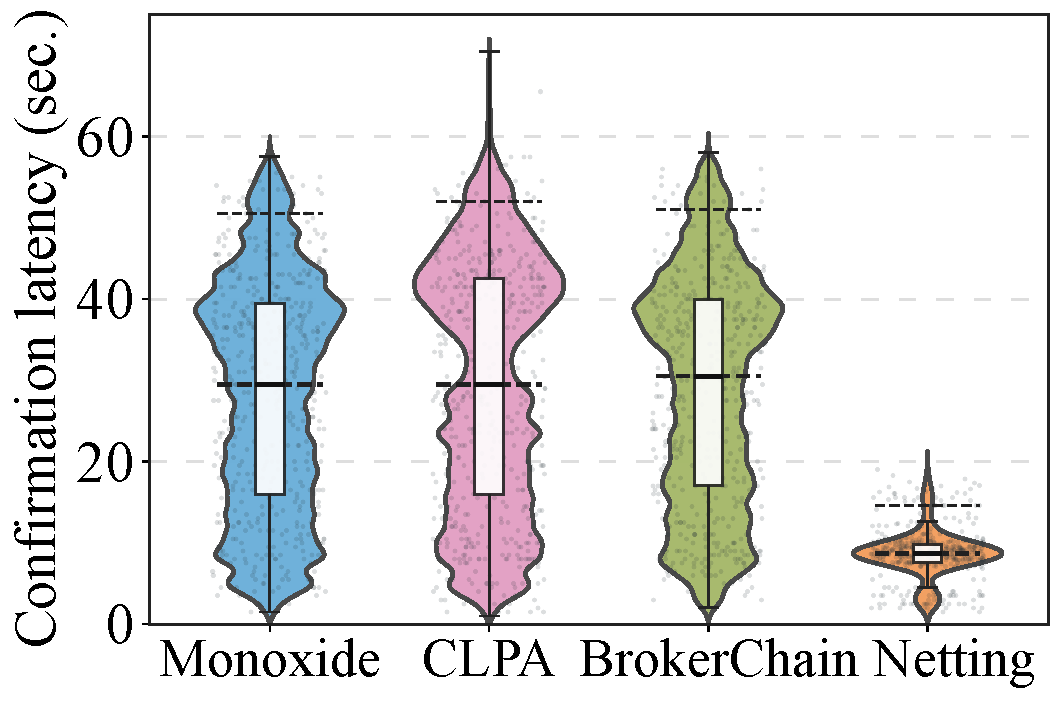
\includegraphics[width=\linewidth]{exp-figs/tx_confirmation_latency_violin.pdf}
    \caption{Confirmation-time distributions.}
    \label{fig:violin}
  \end{subfigure}\hfill
  \begin{subfigure}[t]{0.49\columnwidth}
    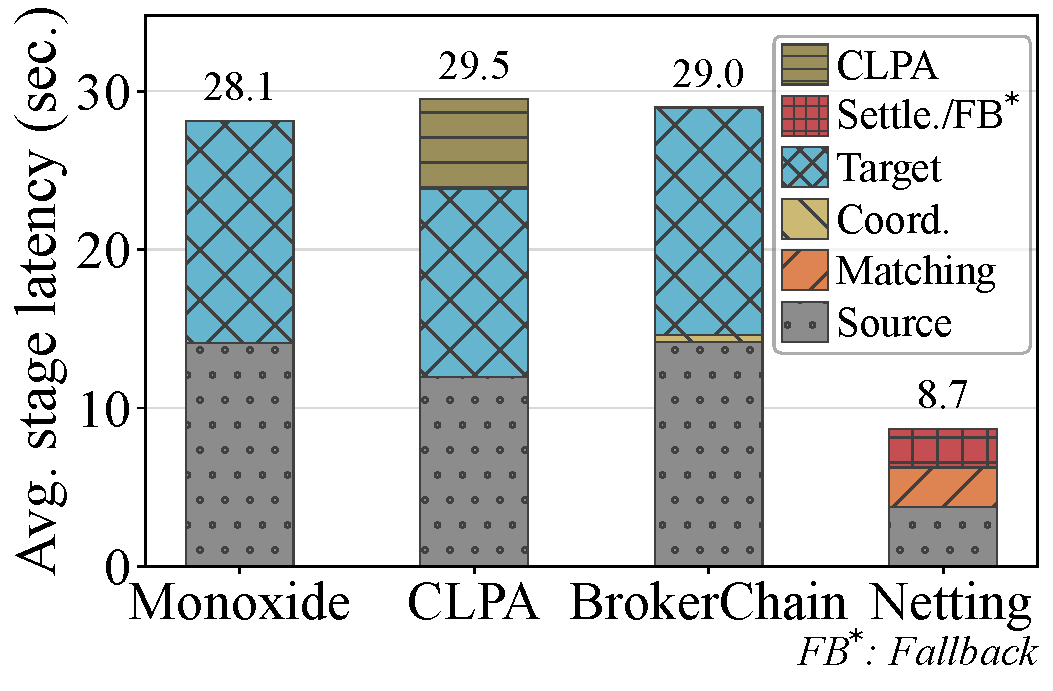
\includegraphics[width=\linewidth]{exp-figs/ctx_stage_latency.pdf}
    \caption{Mean latency by protocol stage.}
    \label{fig:stages}
  \end{subfigure}
  \caption{Eight-shard latency over two 300,000-transaction runs.}
  \label{fig:latency-detail}
\end{figure}

Figure~\ref{fig:violin} shows that \system improves both the center and tail: mean confirmation is 8.69\,s, median 8.67\,s, and p95 14.62\,s. Static relay, broker, and CLPA have means of 28.11, 28.97, and 29.49\,s, with p95 values 50.5--52.0\,s. The shorter upper tail is important for interactive Web3 services, whose user-perceived completion time is dominated by delayed destination execution.

The stage breakdown in Figure~\ref{fig:stages} explains the improvement. \system spends 3.75\,s in source processing, 2.50\,s in coordination, and 2.44\,s in settlement/fallback, totaling 8.69\,s. Static relay spends approximately 14.11\,s at the source and 14.00\,s at the destination. Broker adds 0.40\,s of coordination but still pays 14.38\,s at the destination. Thus the extra matching stage is not free; it is profitable because it replaces far more destination queueing and execution.

\subsection{Q4: Queue pressure}

\begin{figure}[t]
  \centering
  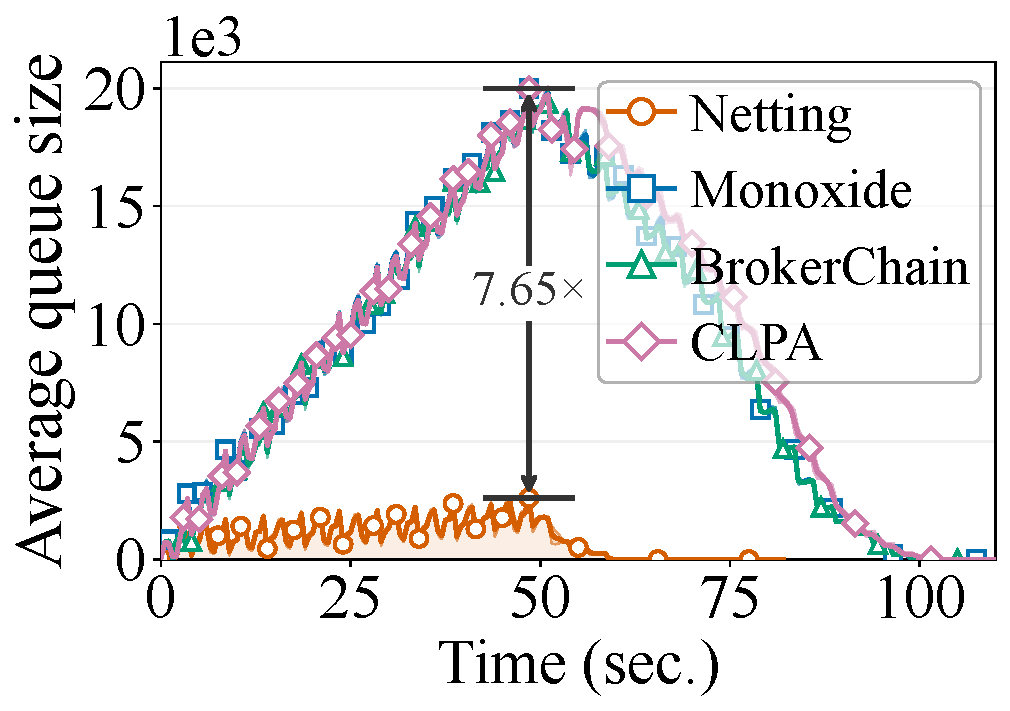
\includegraphics[width=.86\columnwidth]{exp-figs/fig_repeat5_shard8_txpool_mean.pdf}
  \caption{Mean total transaction-pool occupancy at eight shards over five runs. The aggregated path drains destination work faster and avoids the prolonged backlog of transaction-granular baselines.}
  \label{fig:txpool}
\end{figure}

Figure~\ref{fig:txpool} plots total queued work rather than only completed transactions. The baseline pools accumulate and drain slowly because each incoming transfer becomes a destination item. \system's curve peaks lower and returns toward zero earlier. This observation connects the throughput and tail-latency results: aggregation reduces the queue itself, rather than merely prioritizing a subset of transactions.

\subsection{Q5: Sensitivity}

\begin{figure}[t]
  \centering
  \begin{subfigure}[t]{0.49\columnwidth}
    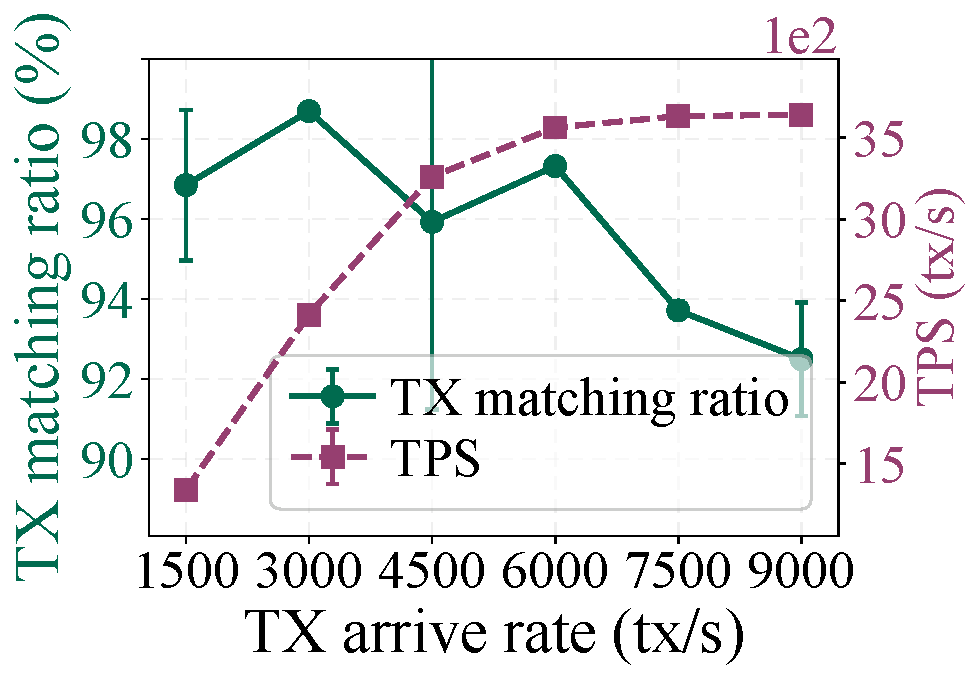
\includegraphics[width=\linewidth]{exp-figs/fig_shard8_ablation_injection_repeat5.pdf}
    \caption{Injection-rate sensitivity.}
    \label{fig:ablation-load}
  \end{subfigure}\hfill
  \begin{subfigure}[t]{0.49\columnwidth}
    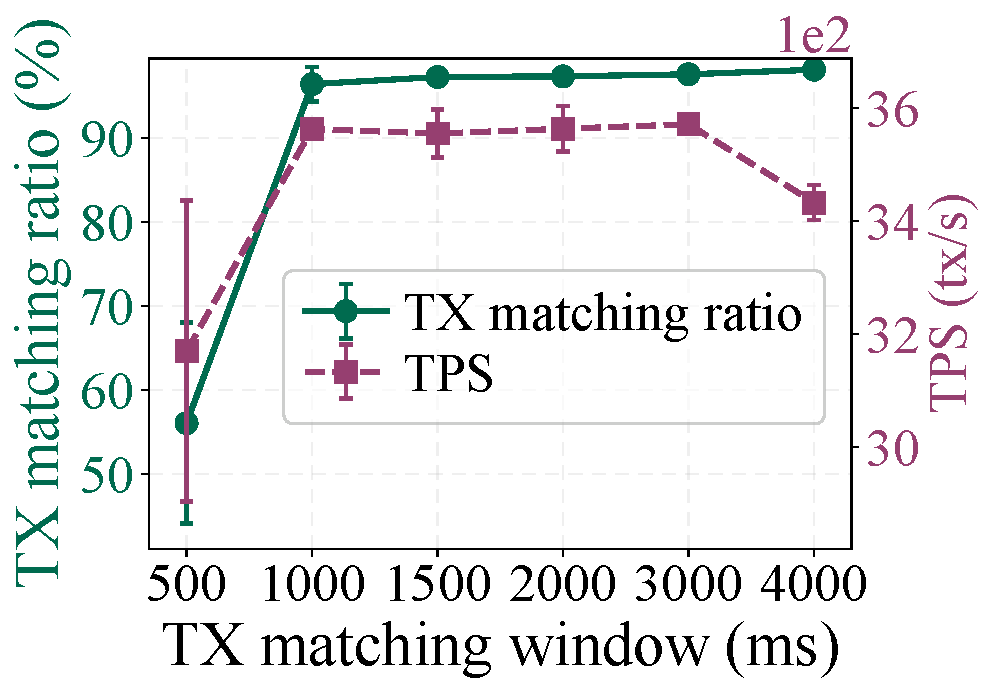
\includegraphics[width=\linewidth]{exp-figs/fig_shard8_ablation_window_repeat5.pdf}
    \caption{Matching-window sensitivity.}
    \label{fig:ablation-window}
  \end{subfigure}
  \caption{Eight-shard sensitivity over five runs. Each panel jointly reports selection, latency, throughput, and source-lock duration.}
  \label{fig:ablation}
\end{figure}

Figure~\ref{fig:ablation-load} varies offered load from 1,500 to 9,000 tx/s. Throughput rises from 1,339 to 3,642 tx/s and then saturates, while mean latency grows from 6.99 to 13.73\,s. Fully selected transaction share stays above 92.5\%, showing that overload affects queueing before it destroys candidate coverage. The matched-value share rises from 21.8\% to roughly 34.7\%, because larger windows expose more opportunities for receiver aggregation.

Figure~\ref{fig:ablation-window} varies the maximum waiting window from 0.5 to 4\,s. A 0.5\,s window selects only 56.0\% on average and yields 14.31\,s latency; at 1--3\,s, selection is 96.4--97.6\%, throughput stays around 3,555--3,571 tx/s, and mean latency remains 8.16--8.99\,s. Extending the window to 4\,s raises matched-value share to 41.9\% but lowers throughput to 3,433 tx/s and increases latency to 9.97\,s. We therefore use a moderate window: waiting longer improves aggregation opportunity but eventually offsets its execution savings.

\subsection{Summary}

The experiments support a consistent mechanism: high selection rates allow many finalized summaries to share destination work; measured matching time is tens of milliseconds; destination queues shrink; and both mean and tail latency fall. The result persists across shard count and load, but the window ablation confirms that coordination must remain bounded.

\section{Related Work}

\paragraph{Cross-shard protocols.}
OmniLedger, RapidChain, and Chainspace established secure sharded execution~\cite{omniledger2018,rapidchain2018,chainspace2018}. Recent systems reduce communication, confirmation, or coordination costs through distributed processing, reliable broadcast, or optimized protocols~\cite{dcchain2024,estuary2024,presto2024,lightcross2024,logos2026,xrbc2026}. Haechi studies cross-shard ordering fairness~\cite{haechi2024}, while Reticulum and Kronos strengthen consensus scalability and resilience~\cite{reticulum2024,kronos2025}. \system is complementary: it reduces the number of receiver-side execution items after source finality.

\paragraph{Broker and placement approaches.}
BrokerChain and Broker2Earn route transfers through intermediaries~\cite{brokerchain2022,broker2earn2024}. SPRING, fine-grained migration, and efficient state sharding improve account placement~\cite{spring2024,finelock2024,statesharding2024}. Those techniques change the route or frequency of cross-shard traffic. \system changes the materialization unit for traffic that remains and does not require broker liquidity or predictable long-term locality.

\paragraph{Batching.}
Conventional batching amortizes ordering or signature verification but may still execute every enclosed transaction. In contrast, \system derives a receiver-delta map and atomically applies it with an inclusion commitment. Its savings therefore include state accesses and destination entries, while its fallback preserves semantics for operations that cannot be aggregated.

\section{Discussion and Limitations}

\paragraph{Workload scope.}
The current fast path covers additive transfers. General smart-contract calls may read shared state, emit ordered events, or revert conditionally, so combining them requires commutativity declarations or application-specific proofs. Such calls safely fall back today.

\paragraph{Coordinator trust and availability.}
The Beacon Chain does not custody value, but it orders selections and certifies settlement. A malicious coordinator can delay service until fallback, not alter certified source effects. A fully decentralized deployment must provision proof data availability and size the Beacon committee independently of transaction shards.

\paragraph{Experimental scope.}
BlockEmulator-X provides repeatable protocol-level comparisons but is not a public wide-area deployment. The current evaluation uses synthetic account transfers and up to 24 shards. WAN faults, fee markets, multi-asset contention, and adversarially skewed receivers remain future work. Moreover, matching-rate metrics depend on the eligibility definition; we therefore report end-to-end throughput, latency, and queue behavior as primary outcomes.

\paragraph{Web implications.}
Receiver aggregation is particularly suitable for Web-facing payment gateways, games, exchanges, and autonomous agents that generate bursts toward shared contracts or merchants. Lower tail confirmation can improve interactive usability, but application interfaces must still expose finality and fallback status rather than promising a fixed completion time.

\section{Conclusion}

\system replaces transaction-granular destination execution with a verifiable pre-matching, matching, aggregation, and settlement pipeline. Source-side finality authorizes compact summaries; pre-matching limits optimizer work; exact selection maximizes covered transactions; aggregation combines receiver deltas across sources; and fallback preserves liveness. In repeated 4--24-shard experiments, this design improves throughput, mean and tail latency, and queue drainage while keeping matching runtime small. The broader lesson is that cross-shard scalability depends not only on faster coordination or better placement, but also on compressing how finalized effects are materialized.

\bibliographystyle{ACM-Reference-Format}
\bibliography{ref}

\appendix
\section{Reproducibility Notes}

The artifact records per-run throughput, confirmation latency, matching runtime, pairwise selection rates, queue occupancy, and stage timestamps. Every scale result reports five runs; the detailed eight-shard latency experiment reports two 300,000-transaction runs. A reproduction should keep consensus size, block interval, injection trace, and network mode identical across methods, and should distinguish selected-transaction share from matched-value share. Settlement and fallback must also share the same consumed-identifier store when checking correctness.

\end{document}
